% TODO Include picture of circuit 3

\FloatBarrier

\begin{figure}[h!]
	\centering
	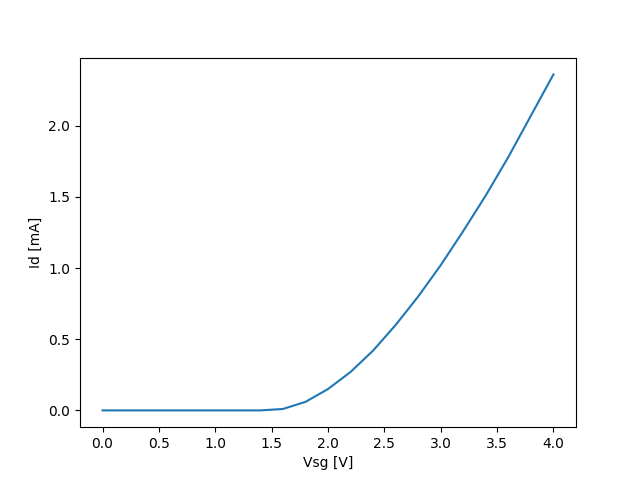
\includegraphics[scale=0.75]{../images/data_3.PNG}
	\caption{$i_{D}$ versus $V_{SG}$ of PMOS where $V_{SB}= 0$\si{\volt}}
	\label{fig:data_3}
\end{figure}

\FloatBarrier

\FloatBarrier

\begin{table}[h!]
	\centering
	\caption{Figure (\ref{fig:data_3}) Data}
	\label{tab:data_3}
	\csvautotabular{../tables/data_3.csv}
\end{table}

\FloatBarrier

As $V_{SG}$ is increased, electrons are repelled from the channel beneath the gate of the PMOS.
This exposes a depletion layer in the channel.
Once $V_{SG}$ hits the threshold voltage $|V_{tp}|$, for which $|V_{tp}| \approx 1.4$\si{\volt} in this case, holes are ripped from the postiviely-charged donor ions in n-type substrate, and a p-type channel is formed. \\

The transistor exits cutoff past $|V_{tp}|$.
If $V_{SD} > V_{SG} - |V_{tp}|$, then the transistor operates in the saturation region.
The drain in this circuit is grounded.
The source is set to supply, which is $V_{DD} = 5$\si{\volt}.
Therefore, $V_{SD} = 5$\si{\volt}.
If $|V_{tp}| \gte 0$ by the definition of the absolute value of a real number.
Therefore, so long as $V_{SG} < V_{SD} + |V_{tp}| \lte 5$\si{\volt}, the transistor stays in saturation.
If $V_{SG}$ is increased past about $4$\si{\volt}, the current in the actual experiment becomes much too large to handle.
As a result, the test cases are limited to $V_{SG} < 4$\si{\volt}.
Thus, by design, the transistor exits cutoff and enters saturation, in which case the current grows with $V_{SG}^{2}$. \\

\FloatBarrier

\begin{figure}[h!]
	\centering
	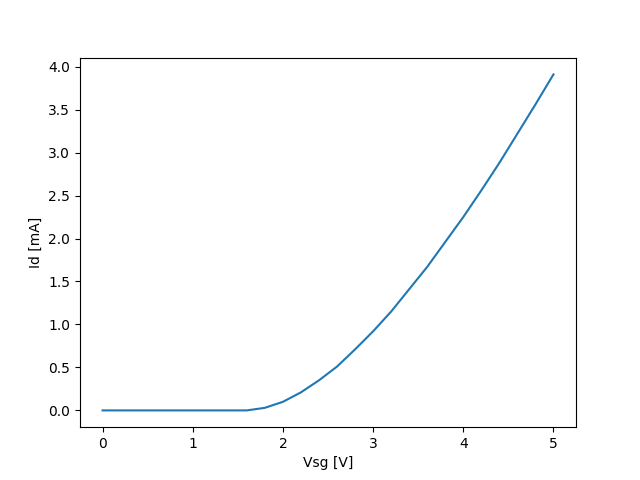
\includegraphics[scale=0.75]{../images/data_3_b.PNG}
	\caption{$i_{D}$ versus $V_{SG}$ of PMOS where $V_{SB}= 0.5$\si{\volt}}
	\label{fig:data_3_b}
\end{figure}

\FloatBarrier

\FloatBarrier

\begin{table}[h!]
	\centering
	\caption{Figure (\ref{fig:data_3_b}) Data}
	\label{tab:data_3_b}
	\csvautotabular{../tables/data_3_b.csv}
\end{table}

\FloatBarrier

When increasing the source-bulk voltage $V_{SB}$, the threshold voltage increases slightly to about $1.6$\si{\volt}.
In a very simplified model, two pn-junction diodes exist in a PMOS transistor.
The first is between the source and the bulk.
The other is between the drain and the bulk.
Initially, the source and bulk voltages are both $5$\si{\volt} relative to ground.
In this situation, because the drain is grounded, a slight reverse saturation current occurs from the bulk to the drain, but no current flows from the source to the bulk.
Now, drop the bulk voltage to $4.5$\si{\volt}, so that $V_{SB} = 0.5$\si{\volt}, while still keeping the source at the supply voltage.
The reverse saturation current in the drain-bulk diode drops slightly, meaning less current flows into the drain.
Moreover, the current from the source to the bulk increases dramatically.
As a result, current is drawn from the source, and less current flows into the drain.
Therefore, less current flows through the channel.
So, a higher $V_{SG}$ is required to achieve the same current.
Thus, the threshold voltage $|V_{tp}|$ must increase.
The transistor exits cutoff around $1.6$\si{\volt} this time.
Therefore, in line with theory, the threshold voltage increased slightly with the increased $V_{SB}$, namely from about $1.4$\si{\volt} to $1.6$\si{\volt}.

% TODO W/L ratio of transistor
